% ****************************************************************************************
% *****************     PRACTICA 1 y 2: TIPOS, MAC Y CHECKSUM     ************************
% ****************************************************************************************


% =======================================================
% =======         HEADER FOR DOCUMENT        ============
% =======================================================
    
    % *********   HEADERS AND FOOTERS ********
    \def\ProjectAuthorLink{https://github.com/SoyOscarRH}           %Just to keep it in line
    \def\ProjectNameLink{https://github.com/CompilandoConocimiento} %Just to keep it in line

    % *********   DOCUMENT ITSELF   **************
    \documentclass[12pt, fleqn]{report}                             %Type of docuemtn and size of font and left eq
    \usepackage[margin = 1.2in]{geometry}                           %Margins and Geometry pacakge
    \usepackage[spanish]{babel}                                     %Please use spanish
    \usepackage[utf8]{inputenc}                                     %Please use spanish - UFT
    \usepackage{ifthen}                                             %Allow simple programming
    \usepackage{hyperref}                                           %Create MetaData for a PDF and LINKS!
    \usepackage{pdfpages}                                           %Create MetaData for a PDF and LINKS!
    \hypersetup{pageanchor = false}                                 %Solve 'double page 1' warnings in build
    \setlength{\parindent}{0pt}                                     %Eliminate ugly indentation
    \author{Oscar Andrés Rosas}                                     %Who I am

    % *********   LANGUAJE AND UFT-8   *********
    \usepackage[T1]{fontenc}                                        %Please use spanish
    \usepackage{textcmds}                                           %Allow us to use quoutes
    \usepackage{changepage}                                         %Allow us to use identate paragraphs
    \usepackage{anyfontsize}                                        %All the sizes

    % *********   MATH AND HIS STYLE  *********
    \usepackage{ntheorem, amsmath, amssymb, amsfonts}               %All fucking math, I want all!
    \usepackage{mathrsfs, mathtools, empheq}                        %All fucking math, I want all!
    \usepackage{cancel}                                             %Negate symbol
    \usepackage{centernot}                                          %Allow me to negate a symbol
    \decimalpoint                                                   %Use decimal point

    % *********   GRAPHICS AND IMAGES *********
    \usepackage{graphicx}                                           %Allow to create graphics
    \usepackage{float}                                              %For images
    \usepackage{wrapfig}                                            %Allow to create images
    \graphicspath{ {Graphics/} }                                    %Where are the images :D

    % *********   LISTS AND TABLES ***********
    \usepackage{listings, listingsutf8}                             %We will be using code here
    \usepackage[inline]{enumitem}                                   %We will need to enumarate
    \usepackage{tasks}                                              %Horizontal lists
    \usepackage{longtable}                                          %Lets make tables awesome
    \usepackage{booktabs}                                           %Lets make tables awesome
    \usepackage{tabularx}                                           %Lets make tables awesome
    \usepackage{multirow}                                           %Lets make tables awesome
    \usepackage{multicol}                                           %Create multicolumns

    % *********   HEADERS AND FOOTERS ********
    \usepackage{fancyhdr}                                           %Lets make awesome headers/footers
    \pagestyle{fancy}                                               %Lets make awesome headers/footers
    \setlength{\headheight}{16pt}                                   %Top line
    \setlength{\parskip}{0.5em}                                     %Top line
    \renewcommand{\footrulewidth}{0.5pt}                            %Bottom line

    \lhead {                                                        %Left Header
        \hyperlink{chapter.\arabic{chapter}}                        %Make a link to the current chapter
        {\normalsize{\textsc{\nouppercase{\leftmark}}}}             %And fot it put the name
    }

    \rhead {                                                        %Right Header
        \hyperlink{section.\arabic{chapter}.\arabic{section}}       %Make a link to the current chapter
            {\footnotesize{\textsc{\nouppercase{\rightmark}}}}      %And fot it put the name
    }
    
    \rfoot{\textsc{\small{\hyperref[sec:Index]{Ve al Índice}}}}     %This will always be a footer  

    \fancyfoot[L]{                                                  %Algoritm for a changing footer
        \ifthenelse{\isodd{\value{page}}}                           %IF ODD PAGE:
            {\href{https://compilandoconocimiento.com/nosotros/}    %DO THIS:
                {\footnotesize                                      %Send the page
                    {\textsc{Oscar Andrés Rosas}}}}                 %Send the page
            {\href{https://compilandoconocimiento.com}              %ELSE DO THIS: 
                {\footnotesize                                      %Send the author
                    {\textsc{Arturo Rivas Rojas}}}}                 %Send the author
    }
    
    
    
% =======================================================
% ===================   COMMANDS    =====================
% =======================================================

    % =========================================
    % =======   NEW ENVIRONMENTS   ============
    % =========================================
    \newenvironment{Indentation}[1][0.75em]                         %Use: \begin{Inde...}[Num]...\end{Inde...}
        {\begin{adjustwidth}{#1}{}}                                 %If you dont put nothing i will use 0.75 em
        {\end{adjustwidth}}                                         %This indentate a paragraph
    \newenvironment{SmallIndentation}[1][0.75em]                    %Use: The same that we upper one, just 
        {\begin{adjustwidth}{#1}{}\begin{footnotesize}}             %footnotesize size of letter by default
        {\end{footnotesize}\end{adjustwidth}}                       %that's it

    \newenvironment{MultiLineEquation}[1]                           %Use: To create MultiLine equations
        {\begin{equation}\begin{alignedat}{#1}}                     %Use: \begin{Multi..}{Num. de Columnas}
        {\end{alignedat}\end{equation}}                             %And.. that's it!
    \newenvironment{MultiLineEquation*}[1]                          %Use: To create MultiLine equations
        {\begin{equation*}\begin{alignedat}{#1}}                    %Use: \begin{Multi..}{Num. de Columnas}
        {\end{alignedat}\end{equation*}}                            %And.. that's it!
    

    % =========================================
    % == GENERAL TEXT & SYMBOLS ENVIRONMENTS ==
    % =========================================
    
    % =====  TEXT  ======================
    \newcommand \Quote {\qq}                                        %Use: \Quote to use quotes
    \newcommand \Over {\overline}                                   %Use: \Bar to use just for short
    \newcommand \ForceNewLine {$\Space$\\}                          %Use it in theorems for example

    % =====  SPACES  ====================
    \DeclareMathOperator \Space {\quad}                             %Use: \Space for a cool mega space
    \DeclareMathOperator \MegaSpace {\quad \quad}                   %Use: \MegaSpace for a cool mega mega space
    \DeclareMathOperator \MiniSpace {\;}                            %Use: \Space for a cool mini space
    
    % =====  MATH TEXT  =================
    \newcommand \Such {\MiniSpace | \MiniSpace}                     %Use: \Such like in sets
    \newcommand \Also {\MiniSpace \text{y} \MiniSpace}              %Use: \Also so it's look cool
    \newcommand \Remember[1]{\Space\text{\scriptsize{#1}}}          %Use: \Remember so it's look cool
    
    % =====  THEOREMS  ==================
    \newtheorem{Theorem}{Teorema}[section]                          %Use: \begin{Theorem}[Name]\label{Nombre}...
    \newtheorem{Corollary}{Colorario}[Theorem]                      %Use: \begin{Corollary}[Name]\label{Nombre}...
    \newtheorem{Lemma}[Theorem]{Lemma}                              %Use: \begin{Lemma}[Name]\label{Nombre}...
    \newtheorem{Definition}{Definición}[section]                    %Use: \begin{Definition}[Name]\label{Nombre}...
    \theoremstyle{break}                                            %THEOREMS START 1 SPACE AFTER

    % =====  LOGIC  =====================
    \newcommand \lIff {\leftrightarrow}                             %Use: \lIff for logic iff
    \newcommand \lEqual {\MiniSpace \Leftrightarrow \MiniSpace}     %Use: \lEqual for a logic double arrow
    \newcommand \lInfire {\MiniSpace \Rightarrow \MiniSpace}        %Use: \lInfire for a logic infire
    \newcommand \lLongTo {\longrightarrow}                          %Use: \lLongTo for a long arrow

    % =====  FAMOUS SETS  ===============
    \DeclareMathOperator \Naturals     {\mathbb{N}}                 %Use: \Naturals por Notation
    \DeclareMathOperator \Primes       {\mathbb{P}}                 %Use: \Primes por Notation
    \DeclareMathOperator \Integers     {\mathbb{Z}}                 %Use: \Integers por Notation
    \DeclareMathOperator \Racionals    {\mathbb{Q}}                 %Use: \Racionals por Notation
    \DeclareMathOperator \Reals        {\mathbb{R}}                 %Use: \Reals por Notation
    \DeclareMathOperator \Complexs     {\mathbb{C}}                 %Use: \Complex por Notation
    \DeclareMathOperator \GenericField {\mathbb{F}}                 %Use: \GenericField por Notation
    \DeclareMathOperator \VectorSet    {\mathbb{V}}                 %Use: \VectorSet por Notation
    \DeclareMathOperator \SubVectorSet {\mathbb{W}}                 %Use: \SubVectorSet por Notation
    \DeclareMathOperator \Polynomials  {\mathbb{P}}                 %Use: \Polynomials por Notation

    % =====  CONTAINERS   ===============
    \newcommand{\Set}[1]{\left\{ \; #1 \; \right\}}                 %Use: \Set {Info} for INTELLIGENT space 
    \newcommand{\bigSet}[1]{\big\{ \; #1 \; \big\}}                 %Use: \bigSet  {Info} for space 
    \newcommand{\BigSet}[1]{\Big\{ \; #1 \; \Big\}}                 %Use: \BigSet  {Info} for space 
    \newcommand{\biggSet}[1]{\bigg\{ \; #1 \; \bigg\}}              %Use: \biggSet {Info} for space 
    \newcommand{\BiggSet}[1]{\Bigg\{ \; #1 \; \Bigg\}}              %Use: \BiggSet {Info} for space 
    
    \newcommand{\Brackets}[1]{\left[ #1 \right]}                    %Use: \Brackets {Info} for INTELLIGENT space
    \newcommand{\bigBrackets}[1]{\big[ \; #1 \; \big]}              %Use: \bigBrackets  {Info} for space 
    \newcommand{\BigBrackets}[1]{\Big[ \; #1 \; \Big]}              %Use: \BigBrackets  {Info} for space 
    \newcommand{\biggBrackets}[1]{\bigg[ \; #1 \; \bigg]}           %Use: \biggBrackets {Info} for space 
    \newcommand{\BiggBrackets}[1]{\Bigg[ \; #1 \; \Bigg]}           %Use: \BiggBrackets {Info} for space 
    
    \newcommand{\Wrap}[1]{\left( #1 \right)}                        %Use: \Wrap {Info} for INTELLIGENT space
    \newcommand{\bigWrap}[1]{\big( \; #1 \; \big)}                  %Use: \bigBrackets  {Info} for space 
    \newcommand{\BigWrap}[1]{\Big( \; #1 \; \Big)}                  %Use: \BigBrackets  {Info} for space 
    \newcommand{\biggWrap}[1]{\bigg( \; #1 \; \bigg)}               %Use: \biggBrackets {Info} for space 
    \newcommand{\BiggWrap}[1]{\Bigg( \; #1 \; \Bigg)}               %Use: \BiggBrackets {Info} for space 

    % =====  BETTERS MATH COMMANDS   =====
    \newcommand{\pfrac}[2]{\Wrap{\dfrac{#1}{#2}}}                   %Use: Put fractions in parentesis

    % =========================================
    % ====   LINEAL ALGEBRA & VECTORS    ======
    % =========================================

    % ===== UNIT VECTORS  ================
    \newcommand{\hati} {\hat{\imath}}                               %Use: \hati for unit vector    
    \newcommand{\hatj} {\hat{\jmath}}                               %Use: \hatj for unit vector    
    \newcommand{\hatk} {\hat{k}}                                    %Use: \hatk for unit vector

    % ===== MAGNITUDE  ===================
    \newcommand{\abs}[1]{\left\lvert #1 \right\lvert}               %Use: \abs{expression} for |x|
    \newcommand{\Abs}[1]{\left\lVert #1 \right\lVert}               %Use: \Abs{expression} for ||x||
    \newcommand{\Mag}[1]{\left| #1 \right|}                         %Use: \Mag {Info} 
    
    \DeclareMathOperator \LinealTransformation {\mathcal{T}}        %Use: \LinealTransformation for a cool T
    \newcommand{\bVec}[1]{\mathbf{#1}}                              %Use for bold type of vector
    \newcommand{\lVec}[1]{\overrightarrow{#1}}                      %Use for a long arrow over a vector
    \newcommand{\uVec}[1]{\mathbf{\hat{#1}}}                        %Use: Unitary Vector Example: $\uVec{i}

    % ===== ALL FOR DOT PRODUCT  =========
    \makeatletter                                                   %WTF! IS THIS
    \newcommand*\dotP{\mathpalette\dotP@{.5}}                       %Use: \dotP for dot product
    \newcommand*\dotP@[2] {\mathbin {                               %WTF! IS THIS            
        \vcenter{\hbox{\scalebox{#2}{$\m@th#1\bullet$}}}}           %WTF! IS THIS
    }                                                               %WTF! IS THIS
    \makeatother                                                    %WTF! IS THIS

    % === WRAPPERS FOR COLUMN VECTOR ===
    \newcommand{\pVector}[1]                                        %Use: \pVector {Matrix Notation} use parentesis
        { \ensuremath{\begin{pmatrix}#1\end{pmatrix}} }             %Example: \pVector{a\\b\\c} or \pVector{a&b&c} 
    \newcommand{\lVector}[1]                                        %Use: \lVector {Matrix Notation} use a abs 
        { \ensuremath{\begin{vmatrix}#1\end{vmatrix}} }             %Example: \lVector{a\\b\\c} or \lVector{a&b&c} 
    \newcommand{\bVector}[1]                                        %Use: \bVector {Matrix Notation} use a brackets 
        { \ensuremath{\begin{bmatrix}#1\end{bmatrix}} }             %Example: \bVector{a\\b\\c} or \bVector{a&b&c} 
    \newcommand{\Vector}[1]                                         %Use: \Vector {Matrix Notation} no parentesis
        { \ensuremath{\begin{matrix}#1\end{matrix}} }               %Example: \Vector{a\\b\\c} or \Vector{a&b&c}

    % === MAKE MATRIX BETTER  =========
    \makeatletter                                                   %Example: \begin{matrix}[cc|c]
    \renewcommand*\env@matrix[1][*\c@MaxMatrixCols c] {             %WTF! IS THIS
        \hskip -\arraycolsep                                        %WTF! IS THIS
        \let\@ifnextchar\new@ifnextchar                             %WTF! IS THIS
        \array{#1}                                                  %WTF! IS THIS
    }                                                               %WTF! IS THIS
    \makeatother                                                    %WTF! IS THIS

    % =========================================
    % =======   FAMOUS FUNCTIONS   ============
    % =========================================

    % == TRIGONOMETRIC FUNCTIONS  ====
    \newcommand{\Cos}[1] {\cos\Wrap{#1}}                            %Simple wrappers
    \newcommand{\Sin}[1] {\sin\Wrap{#1}}                            %Simple wrappers
    \newcommand{\Tan}[1] {tan\Wrap{#1}}                             %Simple wrappers
    
    \newcommand{\Sec}[1] {sec\Wrap{#1}}                             %Simple wrappers
    \newcommand{\Csc}[1] {csc\Wrap{#1}}                             %Simple wrappers
    \newcommand{\Cot}[1] {cot\Wrap{#1}}                             %Simple wrappers

    % === COMPLEX ANALYSIS TRIG ======
    \newcommand \Cis[1]  {\Cos{#1} + i \Sin{#1}}                    %Use: \Cis for cos(x) + i sin(x)
    \newcommand \pCis[1] {\Wrap{\Cis{#1}}}                          %Use: \pCis for the same with parantesis
    \newcommand \bCis[1] {\Brackets{\Cis{#1}}}                      %Use: \bCis for the same with Brackets


    % =========================================
    % ===========     CALCULUS     ============
    % =========================================

    % ====== TRANSFORMS =============
    \newcommand{\FourierT}[1]{\mathscr{F} \left\{ #1 \right\} }     %Use: \FourierT {Funtion}
    \newcommand{\InvFourierT}[1]{\mathscr{F}^{-1}\left\{#1\right\}} %Use: \InvFourierT {Funtion}

    % ====== DERIVATIVES ============
    \newcommand \MiniDerivate[1][x] {\dfrac{d}{d #1}}               %Use: \MiniDerivate[var] for simple use [var]
    \newcommand \Derivate[2] {\dfrac{d \; #1}{d #2}}                %Use: \Derivate [f(x)][x]
    \newcommand \MiniUpperDerivate[2] {\dfrac{d^{#2}}{d#1^{#2}}}    %Mini Derivate High Orden Derivate -- [x][pow]
    \newcommand \UpperDerivate[3] {\dfrac{d^{#3} \; #1}{d#2^{#3}}}  %Complete High Orden Derivate -- [f(x)][x][pow]
    
    \newcommand \MiniPartial[1][x] {\dfrac{\partial}{\partial #1}}  %Use: \MiniDerivate for simple use [var]
    \newcommand \Partial[2] {\dfrac{\partial \; #1}{\partial #2}}   %Complete Partial Derivate -- [f(x)][x]
    \newcommand \MiniUpperPartial[2]                                %Mini Derivate High Orden Derivate -- [x][pow] 
        {\dfrac{\partial^{#2}}{\partial #1^{#2}}}                   %Mini Derivate High Orden Derivate
    \newcommand \UpperPartial[3]                                    %Complete High Orden Derivate -- [f(x)][x][pow]
        {\dfrac{\partial^{#3} \; #1}{\partial#2^{#3}}}              %Use: \UpperDerivate for simple use

    \DeclareMathOperator \Evaluate  {\Big|}                         %Use: \Evaluate por Notation

    % =========================================
    % ========    GENERAL STYLE     ===========
    % =========================================
    
    % =====  COLORS ==================
    \definecolor{RedMD}{HTML}{F44336}                               %Use: Color :D        
    \definecolor{Red100MD}{HTML}{FFCDD2}                            %Use: Color :D        
    \definecolor{Red200MD}{HTML}{EF9A9A}                            %Use: Color :D        
    \definecolor{Red300MD}{HTML}{E57373}                            %Use: Color :D        
    \definecolor{Red700MD}{HTML}{D32F2F}                            %Use: Color :D 

    \definecolor{PurpleMD}{HTML}{9C27B0}                            %Use: Color :D        
    \definecolor{Purple100MD}{HTML}{E1BEE7}                         %Use: Color :D        
    \definecolor{Purple200MD}{HTML}{EF9A9A}                         %Use: Color :D        
    \definecolor{Purple300MD}{HTML}{BA68C8}                         %Use: Color :D        
    \definecolor{Purple700MD}{HTML}{7B1FA2}                         %Use: Color :D 

    \definecolor{IndigoMD}{HTML}{3F51B5}                            %Use: Color :D        
    \definecolor{Indigo100MD}{HTML}{C5CAE9}                         %Use: Color :D        
    \definecolor{Indigo200MD}{HTML}{9FA8DA}                         %Use: Color :D        
    \definecolor{Indigo300MD}{HTML}{7986CB}                         %Use: Color :D        
    \definecolor{Indigo700MD}{HTML}{303F9F}                         %Use: Color :D 

    \definecolor{BlueMD}{HTML}{2196F3}                              %Use: Color :D        
    \definecolor{Blue100MD}{HTML}{BBDEFB}                           %Use: Color :D        
    \definecolor{Blue200MD}{HTML}{90CAF9}                           %Use: Color :D        
    \definecolor{Blue300MD}{HTML}{64B5F6}                           %Use: Color :D        
    \definecolor{Blue700MD}{HTML}{1976D2}                           %Use: Color :D        
    \definecolor{Blue900MD}{HTML}{0D47A1}                           %Use: Color :D  

    \definecolor{CyanMD}{HTML}{00BCD4}                              %Use: Color :D        
    \definecolor{Cyan100MD}{HTML}{B2EBF2}                           %Use: Color :D        
    \definecolor{Cyan200MD}{HTML}{80DEEA}                           %Use: Color :D        
    \definecolor{Cyan300MD}{HTML}{4DD0E1}                           %Use: Color :D        
    \definecolor{Cyan700MD}{HTML}{0097A7}                           %Use: Color :D        
    \definecolor{Cyan900MD}{HTML}{006064}                           %Use: Color :D 

    \definecolor{TealMD}{HTML}{009688}                              %Use: Color :D        
    \definecolor{Teal100MD}{HTML}{B2DFDB}                           %Use: Color :D        
    \definecolor{Teal200MD}{HTML}{80CBC4}                           %Use: Color :D        
    \definecolor{Teal300MD}{HTML}{4DB6AC}                           %Use: Color :D        
    \definecolor{Teal700MD}{HTML}{00796B}                           %Use: Color :D        
    \definecolor{Teal900MD}{HTML}{004D40}                           %Use: Color :D 

    \definecolor{GreenMD}{HTML}{4CAF50}                             %Use: Color :D        
    \definecolor{Green100MD}{HTML}{C8E6C9}                          %Use: Color :D        
    \definecolor{Green200MD}{HTML}{A5D6A7}                          %Use: Color :D        
    \definecolor{Green300MD}{HTML}{81C784}                          %Use: Color :D        
    \definecolor{Green700MD}{HTML}{388E3C}                          %Use: Color :D        
    \definecolor{Green900MD}{HTML}{1B5E20}                          %Use: Color :D

    \definecolor{AmberMD}{HTML}{FFC107}                             %Use: Color :D        
    \definecolor{Amber100MD}{HTML}{FFECB3}                          %Use: Color :D        
    \definecolor{Amber200MD}{HTML}{FFE082}                          %Use: Color :D        
    \definecolor{Amber300MD}{HTML}{FFD54F}                          %Use: Color :D        
    \definecolor{Amber700MD}{HTML}{FFA000}                          %Use: Color :D        
    \definecolor{Amber900MD}{HTML}{FF6F00}                          %Use: Color :D

    \definecolor{BlueGreyMD}{HTML}{607D8B}                          %Use: Color :D        
    \definecolor{BlueGrey100MD}{HTML}{CFD8DC}                       %Use: Color :D        
    \definecolor{BlueGrey200MD}{HTML}{B0BEC5}                       %Use: Color :D        
    \definecolor{BlueGrey300MD}{HTML}{90A4AE}                       %Use: Color :D        
    \definecolor{BlueGrey700MD}{HTML}{455A64}                       %Use: Color :D        
    \definecolor{BlueGrey900MD}{HTML}{263238}                       %Use: Color :D        

    \definecolor{DeepPurpleMD}{HTML}{673AB7}                        %Use: Color :D

    \newcommand{\Color}[2]{\textcolor{#1}{#2}}                      %Simple color environment
    \newenvironment{ColorText}[1]                                   %Use: \begin{ColorText}
        { \leavevmode\color{#1}\ignorespaces }                      %That's is!

    % =====  CODE EDITOR =============
    \lstdefinestyle{CompilandoStyle} {                              %This is Code Style
        backgroundcolor     = \color{BlueGrey900MD},                %Background Color  
        basicstyle          = \tiny\color{white},                   %Style of text
        commentstyle        = \color{BlueGrey200MD},                %Comment style
        stringstyle         = \color{Green300MD},                   %String style
        keywordstyle        = \color{Blue300MD},                    %keywords style
        numberstyle         = \tiny\color{TealMD},                  %Size of a number
        frame               = shadowbox,                            %Adds a frame around the code
        breakatwhitespace   = true,                                 %Style   
        breaklines          = true,                                 %Style   
        showstringspaces    = false,                                %Hate those spaces                  
        breaklines          = true,                                 %Style                   
        keepspaces          = true,                                 %Style                   
        numbers             = left,                                 %Style                   
        numbersep           = 10pt,                                 %Style 
        xleftmargin         = \parindent,                           %Style 
        tabsize             = 4,                                    %Style
        inputencoding       = utf8/latin1                           %Allow me to use special chars
    }
 
    \lstset{style = CompilandoStyle}                                %Use this style







% =====================================================
% ============        COVER PAGE       ================
% =====================================================
\begin{document}
\begin{titlepage}
    
    % ============ TITLE PAGE STYLE  ================
    \definecolor{TitlePageColor}{cmyk}{1,.60,0,.40}                 %Simple colors
    \definecolor{ColorSubtext}{cmyk}{1,.50,0,.10}                   %Simple colors
    \newgeometry{left=0.20\textwidth}                               %Defines an Offset
    \pagecolor{TitlePageColor}                                      %Make it this Color to page
    \color{white}                                                   %General things should be white

    % ===== MAKE SOME SPACE =========
    \vspace                                                         %Give some space
    \baselineskip                                                   %But we need this to up command

    % ============ NAME OF THE PROJECT  ============
    \makebox[0pt][l]{\rule{1.3\textwidth}{3pt}}                     %Make a cool line
    
    \href{https://compilandoconocimiento.com}                       %Link to project
    {\textbf{\textsc{\Huge ESCOM - IPN}}}\\[2.7cm]                  %Name of project   

    % ============ NAME OF THE BOOK  ===============
    \href{\ProjectNameLink/LibroAnalisisDeAlgoritmos}               %Link to Author
    {\fontsize{35}{40}                                              %Size of the book
        \selectfont
        \textbf{Reporte Practica 1 y 2: \\[0.5cm]  }}
    {\fontsize{15}{20}                                              %Size of the book
        \selectfont
        \textbf{Tipo de Trama, Dirección MAC y diferentes Checksums}}\\[0.5cm]     %Name of the book
    \textcolor{ColorSubtext}                                        %Color or the topic
        {\textsc{\LARGE Redes de Computadora}}                           %Name of the general theme
    
    \vfill                                                          %Fill the space
    
    % ============ NAME OF THE AUTHOR  =============
    \href{\ProjectAuthorLink}                                       %Link to Author
    {\LARGE 
    \textsf{Oscar Andrés Rosas Hernandez y Arturo Rivas Rojas}}   %Author

    % ===== MAKE SOME SPACE =========
    \vspace                                                         %Give some space
    \baselineskip                                                   %But we need this to up command
    
    {\large \textsf{Realizada Marzo 2018}}                          %Date
    
    {\large \textsf{Entregada 23 de Marzo 2018}}                    %Date

\end{titlepage}


% =====================================================
% ==========      RESTORE TO DOCUMENT      ============
% =====================================================
\restoregeometry                                                    %Restores the geometry
\nopagecolor                                                        %Use to restore the color to white




% =====================================================
% ========                INDICE              =========
% =====================================================
\tableofcontents{}
\label{sec:Index}

\clearpage



% ===============================================================================
% ===================          MARCO TEORICO               ======================
% ===============================================================================
\chapter{Marco Teórico}

    


    % ==============================================================================
    % =========================       ETHERNET              ========================
    % ==============================================================================
    \clearpage
    \section{Protocolo Ethernet}

            \begin{figure}[h]
                \centering
                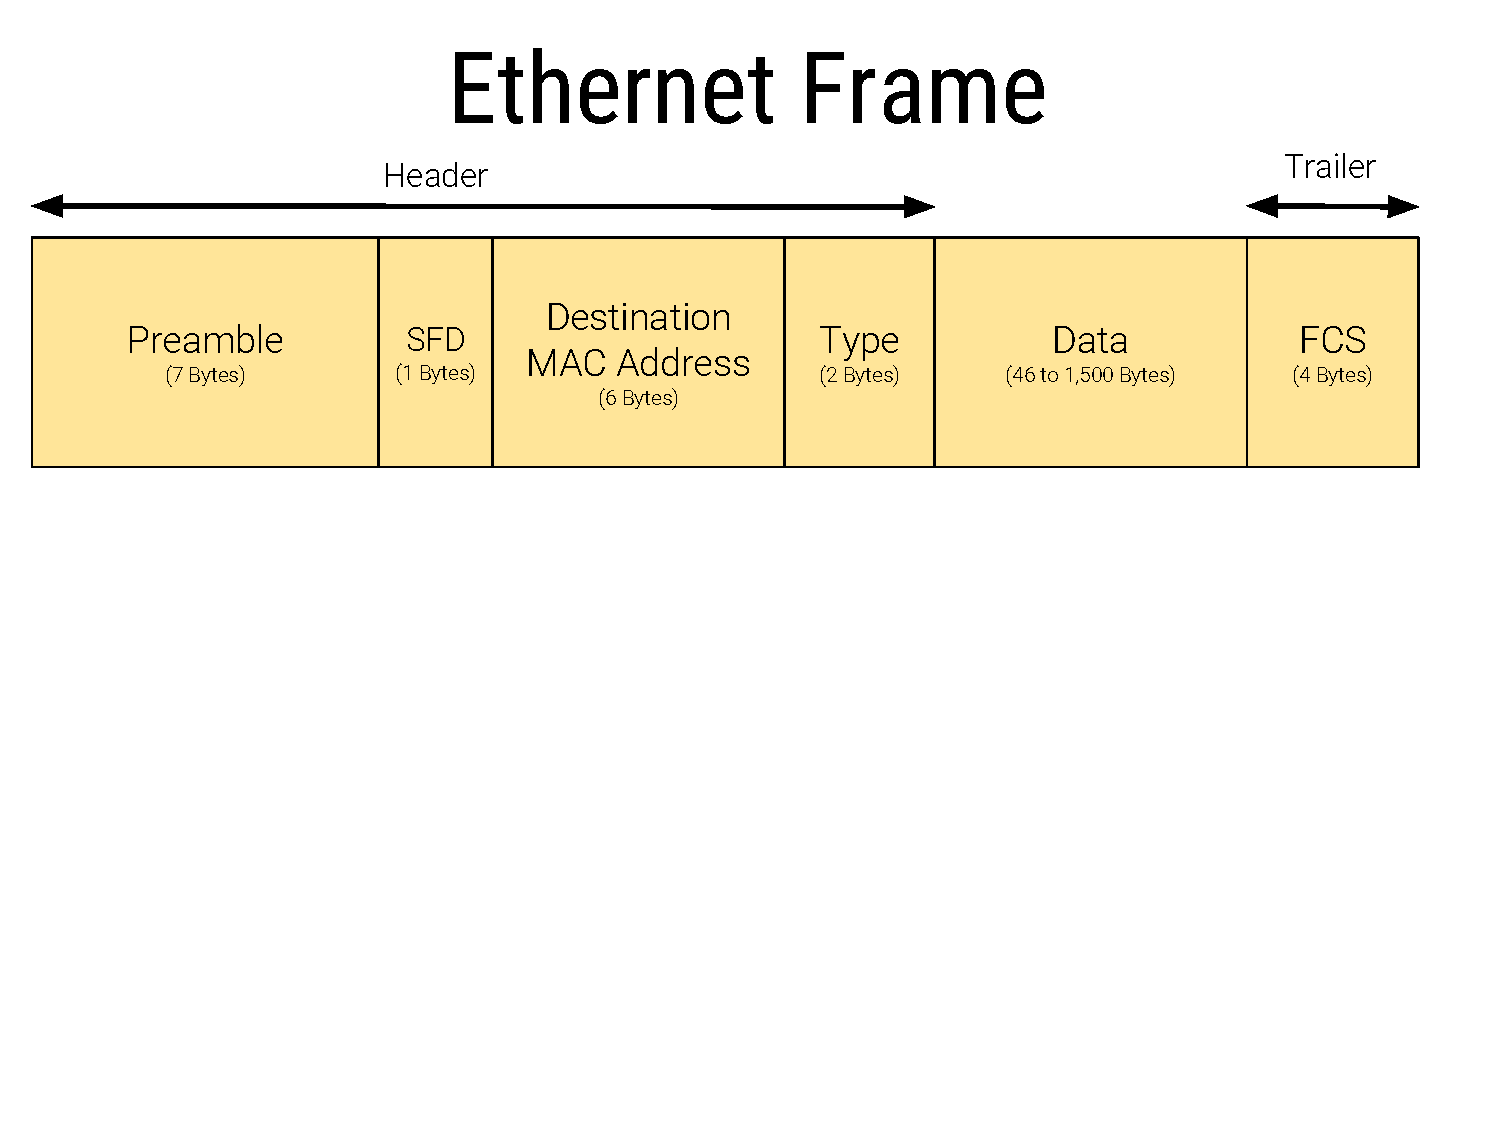
\includegraphics[width=0.85\textwidth]{Ethernet-Header}
            \end{figure}

            % ==============================================================
            % =================       EXPLICACION         ==================
            % ==============================================================
            \subsection{Explicación}

                Los campos que componen una trama ethernet son los siguientes: 

                \begin{itemize}
                    
                    \item 
                        \textbf{Preámbulo (Preamble)} 

                            Campo con una secuencia de bits utilizada para sincronizar y
                            estabilizar el medio físico antes de iniciar la transmisión.
                            Es una secuencia de unos y ceros. conocida que permite a los
                            nodos saber que esta llegando un nuevo frame.

                            El patrón es el siguiente:

                            \Color{Blue900MD}{$10101010 10101010 10101010 10101010 10101010 10101010 10101010$} 

                            \emph{Tamaño: 7 Bytes} 

                    \item
                        \textbf{SFD (Start Frame Delimiter)} 

                            Delimitador de inicio de trama. Campo que contiene la
                            secuencia \Color{Red700MD}{$10101011$}.

                            Indica el inicio de una trama de datos.

                            \emph{Tamaño: 1 Byte} 

                    \item
                        \textbf{Dirección de Destino (Destination Address)}
 
                            Campo que contiene la dirección MAC a la que se envía la trama.

                            El bit más a la izquierda del campo indica cuando la dirección es individual (indicado por un 0)
                            o un grupo de direcciones (indicado por un 1).
                            El segundo bit desde la izquierda indica cuando la dirección destino es globalmente administrada
                            (indicado por un 0). 
                            La capa de enlace de datos del remitente añade la dirección de destino a la trama.
                            La capa de enlace de datos del destinatario examina la dirección de destino para identificar
                            los mensajes a recibir. 

                            \emph{Tamaño: 6 Bytes} 

                    \clearpage

                    \item
                        \textbf{Dirección de Origen (Source Address)}

                            Campo que contiene la dirección MAC del dispositivo que envía la trama.
                            La dirección de origen es siempre una dirección individual y el bit más a la izquierda es
                            siempre 0.
                            Con ella el receptor conoce a quien debe dirigir las respuestas del mensaje. 
                            
                            \emph{Tamaño: 6 Bytes} 

                    \item
                        \textbf{Tipo de Protocolo o Longitud}

                            Este campo es el que distingue a las tramas IEEE 802.3 de las tramas Ethernet. 

                            Valores para este campo iguales o menores de x05DC (1500 en decimal) indican que es una trama IEEE 802.3 y
                            el valor representa la longitud del campo de datos. 

                            Valores para este campo iguales o mayores de x0600 indican que es una trama Ethernet y el valor representa
                            el tipo de protocolo. 

                            \emph{Tamaño: 2 Bytes} 

                    \item
                        \textbf{Datos and Pad(Payload)}

                        Contiene los datos a transferir entre origen y destino.
                        Si este campo fuera menor de 46 bytes se añade un campo de \Quote{relleno}, es decir pad para mantener
                        el tamaño mínimo de paquete.

                        \emph{Tamaño: 46 a 1,500 Bytes} 


                    \item
                        \textbf{FCS (Frame Check Sequence)}

                        Secuencia de verificación de trama. 

                        Campo que contiene un valor de para control de errores, CRC (Cyclical Redundancy Check).
                        La verificación de redundancia cíclica (CRC), consiste en un valor calculado por el emisor que resume todos
                        los datos de la trama.
                        El receptor calcula nuevamente el valor y, si coincide con el de la trama, entiende que la trama se ha

                        El campo FCS es generado ó calculado sobre los campos dirección de destino, la dirección de origen,
                        el tipo/longitud y datos. 
                        
                        \emph{Tamaño: 4 Bytes} 

                \end{itemize}



    % ==============================================================
    % =================       DEFINICIONES        ==================
    % ==============================================================
    \clearpage
    \section{Suma de Comprobación: CheckSum}

        Este algoritmo permite verificar la integridad de la PDU y su calculo es de la siguiente manera:

        \begin{itemize}
            \item Ordena los datos en palabras de 16 bits
            \item Poner ceros en la posición del checksum y sumar con acarreos
            \item Suma cualquier acarreo fuera de los 16 bits
            \item Complementar a uno
        \end{itemize}


    % ===============================================================================
    % ======================      PROTOCOLO IP         ==============================
    % ===============================================================================
    \section{Protocolo IP}


        % ==============================================================
        % =================       DEFINICIONES        ==================
        % ==============================================================
        \subsection{Definiciones}

            Debido a la cantidad de cables necesarios para conectar cada red con cada otra red del mundo
            no todas las redes tienen una conexión directa, es decir, no existe un cable entre tu red
            lócal y los servidores de Facebook por ejemplo.

            Por eso existe el Protocolo IP que nos permite comunicarnos entre redes.

            En resumén lo que permite es que tu red local solo este conectada a unas pocas redes y a
            varios routers, estos tienen algo llamado una tabla de direcciones, que les permite navegar
            entre redes hasta encontrar su destino. 

            El enrutamiento es parecido a la recursión, en el sentido en que no soluciona tu problema
            sino que solo te lleva un paso más cerca.


            % ==============================================================
            % =================       DIRECCION IP        ==================
            % ==============================================================
            \subsubsection{Direcciones IP}

                Es un identificador único (o casi, ya verás después porque). Necesitamos
                un identificador único porque es lo que nos permite enviar información y que 
                la información que esperamos de regreso sepa a donde llegar.



        % ==============================================================
        % =================     DIRECCION IPv4        ==================
        % ==============================================================
        \clearpage
        \subsection{Dirección IPv4}

            Como fue originalmente desarrollado este esquema podría alocar un identificador
            de \textbf{32 bits} a cada dispositivo que se quisiera conectar a internet.
            Esto nos daría algo así como 4 mill millones de posibles direcciones IP.

            La convención es que estos serían representados como 4 conjuntos de 8 bits representados
            en decimal (una forma un poquito más amigable al público general), es decir:

            \begin{figure}[h]
                \centering
                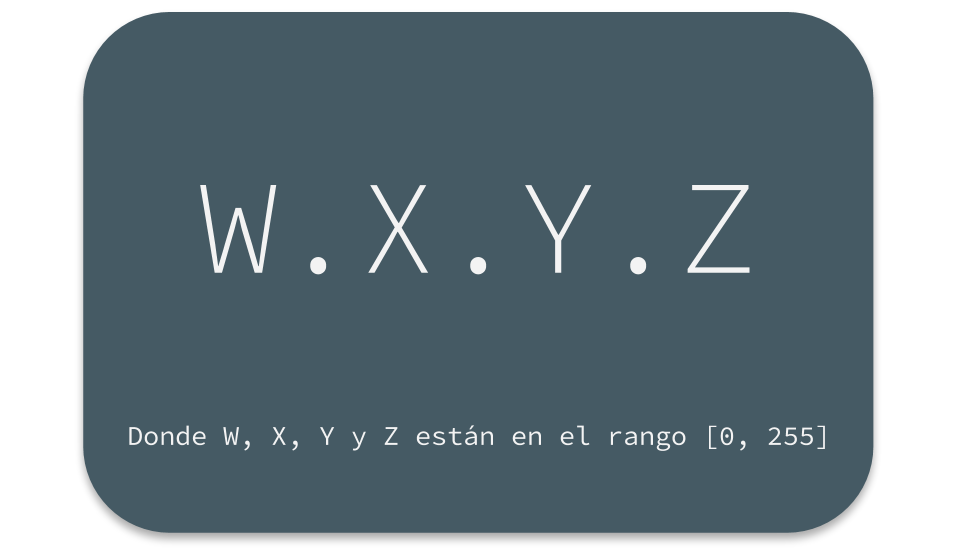
\includegraphics[width=0.80\textwidth]{IPv4}
            \end{figure}

            Por ejemplo una IP v4 válida podría ser $140.247.220.12$. 


            % =========================================================
            % =========   PROBLEMAS CON IP  V4    =====================
            % =========================================================
            \vspace{1.5em}
            \subsection{Problemas con IPv4}

                Ahora, recuerda que te dige que IP v4 acepta unos 4 mil millones de direcciones
                válidas, ahora el problema es que ahora mismo hay vivos mas de 7 mil millones
                de personas (A principios del siglo XXI) cada una con seguramente más de un
                dispositivo que quieran conectar a internet.

                Por lo tanto tenemos que encontrar una forma de solucionar esto.



    % ==============================================================================
    % =========================       TCP                 ==========================
    % ==============================================================================
    \clearpage
    \section{Protocolo TCP}



        % ==============================================================
        % =================       HEADER DEL TCP      ==================
        % ==============================================================
        \subsection{Header - Encabezado}

            \begin{figure}[h]
                \centering
                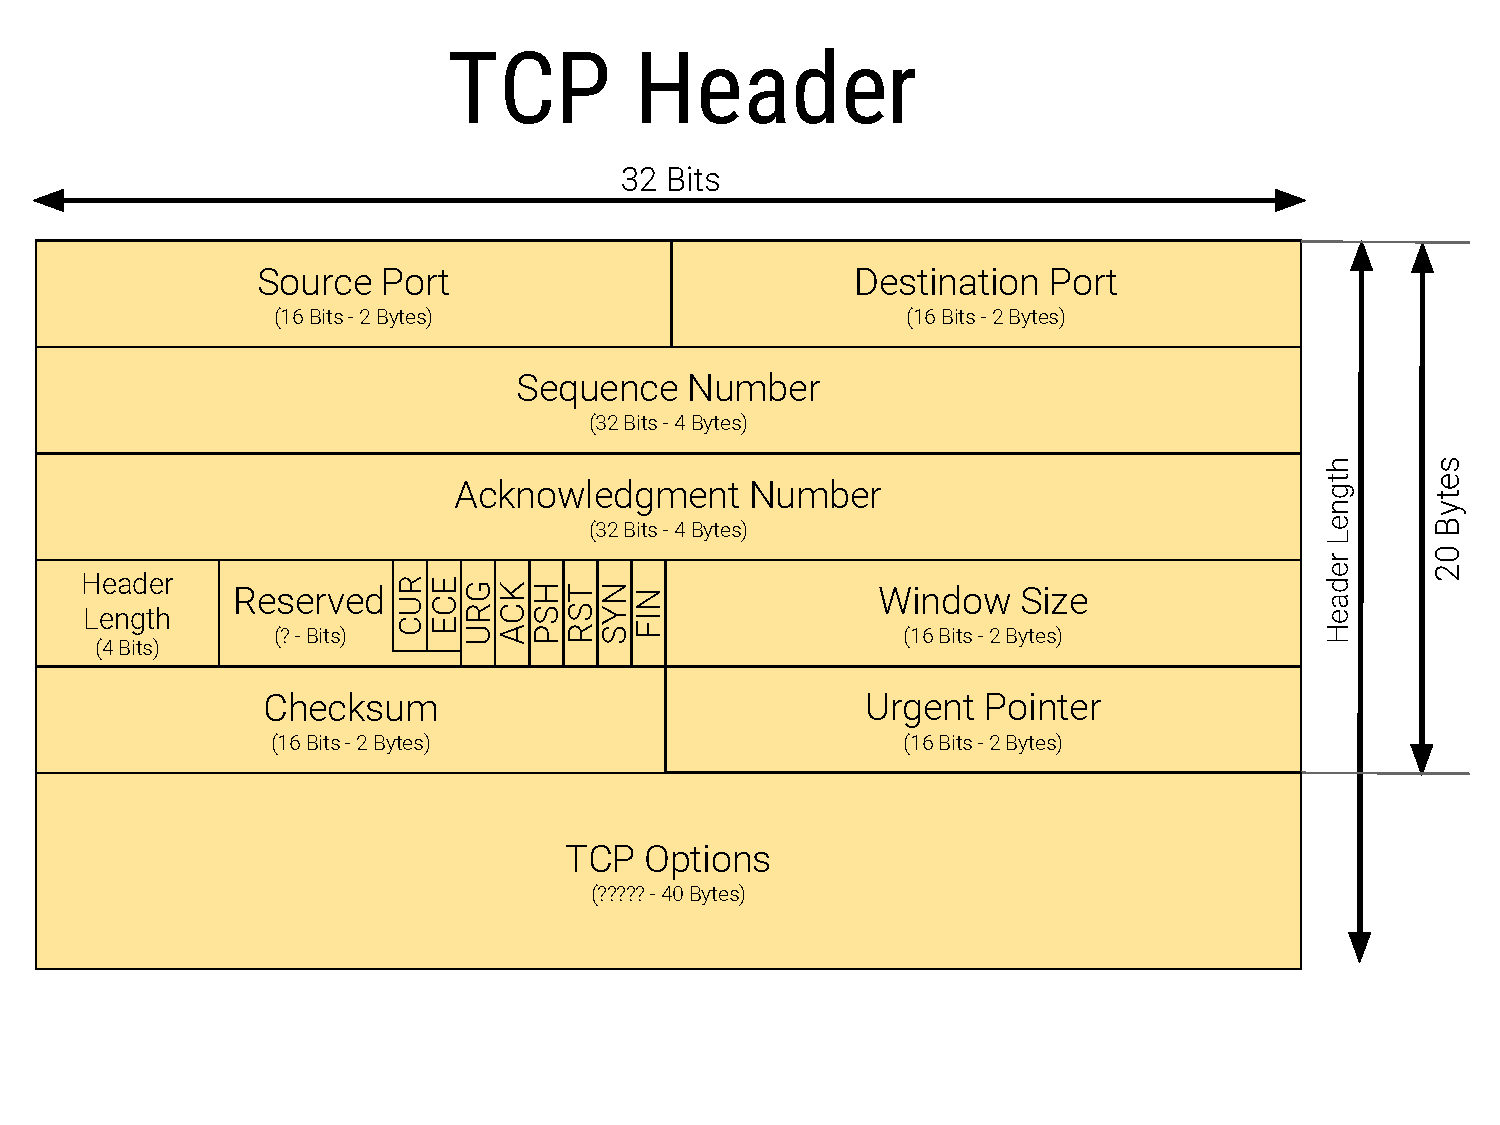
\includegraphics[width=0.95\textwidth]{TCP-Header}
            \end{figure}




% ===============================================================================
% ===================          MARCO TEORICO               ======================
% ===============================================================================
\chapter{Practica 1}


    % ===============================================================================
    % ===================          DESARROLLO                  ======================
    % ===============================================================================
    \section{Desarrollo}

        La práctica consiste en capturar tramas que pasan a través de la tarjeta de red configurada
        en modo promiscuo. A partir de estas tramas analizamos si se trataba de una trama Ethernet,
        y posteriormente si el protocolo de Internet era IP. Para ello utilizamos la librería pcap
        y el código que nos fue proporcionado por el profesor. 

        Ahora procediamos con la parte inreresante, encontrar las direcciones MAC de origen y destino
        así como el tipo de red de cada una de las tramas analizadas, para hacerlo usabamos el siguiente
        algoritmo.

        \begin{enumerate}
            \item Creabamos dos variables temporables que almacenarias las direcciones mac así como una
            tercera que sería el tipo.

            \item
                Para encontrar la MAC de origen lo que haciamos es que contabamos los primeros 6 bytes de
                la trama y los añadiamos uno por uno a la variable temporal, de una manera parecida
                con lo siguientes 6 para la MAC destino.

            \item
                Para encontrar el tipo tendríamos que usar algo de aritmetica de corrimiento para
                obtener el número formado por los bytes 12, 13

            \item 
                Finalmente procediamos a mostrarlo por pantalla los 3 resultados
        \end{enumerate}


    % ===============================================================================
    % ===================          DESARROLLO                  ======================
    % ===============================================================================
    \clearpage
    \section{Capturas}

        \begin{figure}[h]
            \centering
            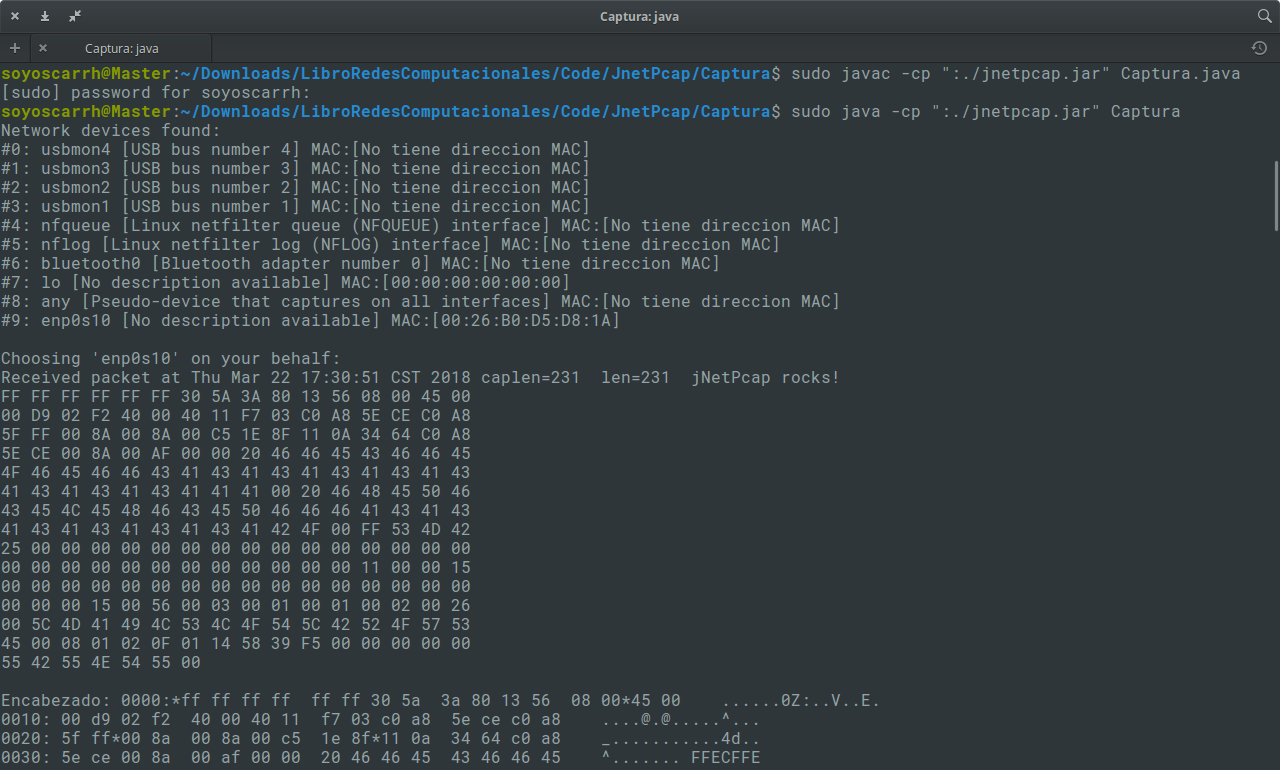
\includegraphics[width=0.85\textwidth]{Captura1}

            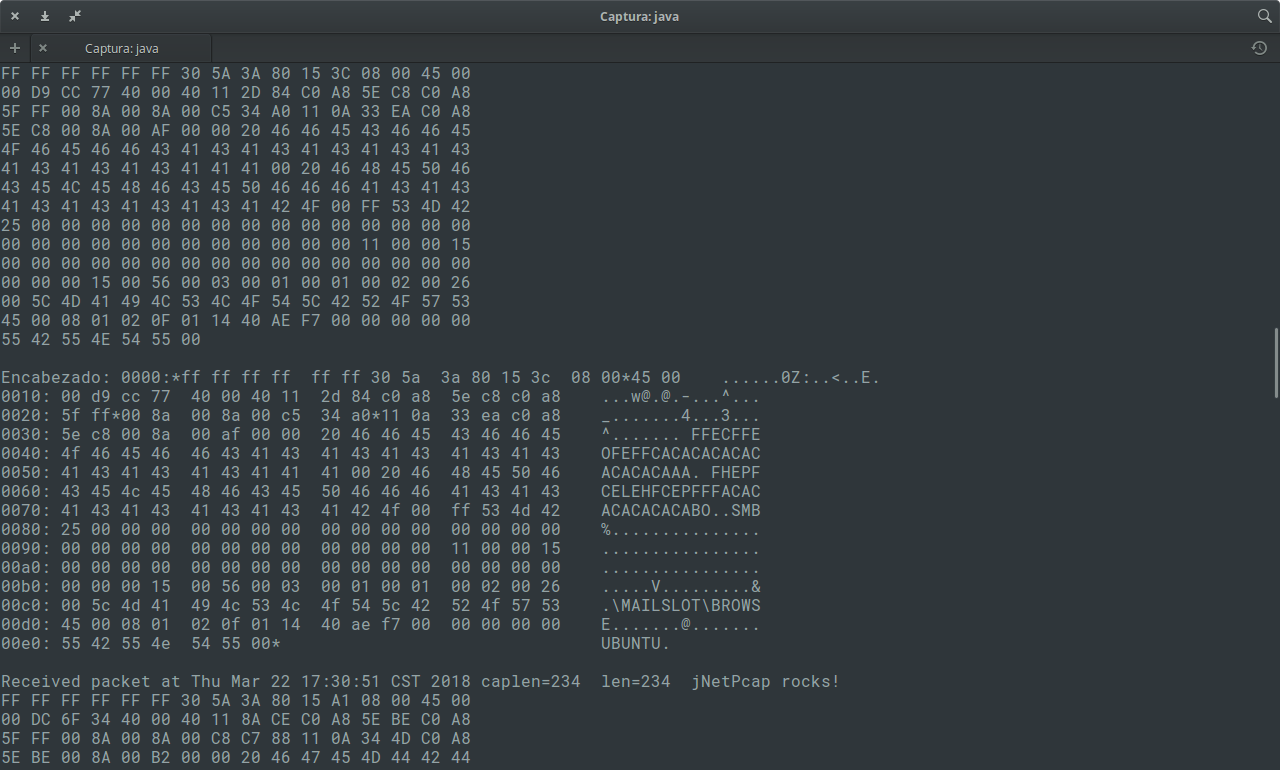
\includegraphics[width=0.85\textwidth]{Captura2}
        \end{figure}



    % ===============================================================================
    % ===================          CODIGO                      ======================
    % ===============================================================================
    \clearpage
    \section{Código}

        \lstinputlisting[language=Java, linerange={162, 270}, gobble=8]{Code/Checksumv2.java}


    % ===============================================================================
    % ===================          CONCLUSIONES                ======================
    % ===============================================================================
    \clearpage
    \section{Conclusiones}

        \textbf{Arturo Rivas Rojas}: 

            La práctica fue realmente enriquecedora en cuanto a los temas del curso,
            ya que me ayudo a entender las bases de como van a ser las practicas posteriores, sobretodo
            en el uso de las biblioteca PCAP que fueron el 90\% de los problemas de esta practica,
            lograr que todo el sistema funcionara a la perfección.


            También por otro lado, me proporciono claridad sobre como es que podemos pasar
            de lo que vemos teoricamente a un codigo real y a aplicaciones de la vida real.

        \textbf{Rosas Hernandez Oscar Andrés}: 

            Es esta práctica implementamos, gracias a la biblioteca PCAP como es que podemos obtener
            y mostrar todo la información cruda que obtuvimos al hacer que nuestra tarjeta se ponga
            a recibir tramas en un modo promiscuo.

            Vimos ademas como es que podemos obtener 3 elementos clave de dichas trama, primeramente
            las dirrecciones MACa, despues como es que tenemos que hacer algo de aritemetica con los
            corrientos para poder obtner e tipo, lo cual resultará un campo super importante
            en futuras practicas.



% ===============================================================================
% ===================          MARCO TEORICO               ======================
% ===============================================================================
\chapter{Practica 2}


    % ===============================================================================
    % ===================          DESARROLLO                  ======================
    % ===============================================================================
    \clearpage
    \section{Desarrollo}

        La práctica consiste en capturar tramas que pasan a través de la tarjeta de red configurada
        en modo promiscuo. A partir de estas tramas analizamos si se trataba de una trama Ethernet,
        y posteriormente si el protocolo de Internet era IP. Para ello utilizamos la librería pcap
        y el código que nos fue proporcionado por el profesor. 

        Para esta práctica supusimos que la trama con la que se trataba era Ethernet, por lo cual
        no se revisó que el campo tipo/longitud fuera mayor o igual a 1500 bytes. 

        Posteriormente, revisamos el byte 13 y 14 de la trama para verificar que el protocolo que
        se iba a utilizar era IPv4, es decir, revisamos que el valor fuera igual a 0x08 en el byte
        13 y 0x00en el byte 14. 

        Una vez validado el tipo de protocolo como IPv4 continuamos a calcular el checksum para
        verificar posibles errores y dar por buena la trama. 

        El procedimiento que seguimos fue el siguiente:
        \begin{enumerate}
            \item Calcular la longitud del encabezado IP. 
            \item Crear un nuevo arreglo de bytes para almacenar el encabezado. 
            \item Identificar IP de origen e IP destino. 
            \item Calcular el checksum utilizando el método proporcionado por el profesor. 
        \end{enumerate}

        Finalmente, procedimos a identificar el protocolo que se utilizó en la capa de transporte
        Para esto revisamos el valor del byte 24 de la trama. Si el valor resultaba ser 0x06,
        sabíamos que se trataba de TCP. Por otro lado, si el valor era 0x11, el protocolo era UDP. 

        Para ambos casos se requería calcular el valor del checksum. Sin embargo, para ambos
        había que calcular previamente un pseudo-header que se utiliza en el cálculo del checksum. 

        En cuanto al checksum de TCP, lo calculamos de la manera siguiente: 

        \begin{enumerate}
            \item Calculamos la longitud del encabezado TCP. 
            \item Creamos un nuevo arreglo que almacenaba el encabezado TCP. 
            \item Creamos un arreglo que iba a contener la información correspondiente al pseudo-header. 
            \item Agregamos la IP de origen y destino al pseudo-header, en ese orden. 
            \item Agregamos la información correspondiente a los bytes 9 y 10. 
                En el byte 9 se asigna el valor de 0 y en el byte 10 el valor
                de 0x06 correspondiente a que se trata de un protocolo TCP. 
            \item Calculamos la longitud del payload utilizando la longitud total
                menos la longitud del encabezado IP menos 14 que es la longitud del
                encabezado TCP. 
            \item Agregamos la información del payload a los bytes 11 y 12. 
            \item Creamos un nuevo arreglo que contendrá el payload de TCP y copiamos la información. 
            \item Creamos un arreglo auxiliar que contendrá: el pseudo-header, el encabezado TCP y el payload. 
            \item Calculamos el checksum utilizando el arreglo auxiliar. 
        \end{enumerate}

        Por otra parte el checksum de UPD, lo calculamos de la manera siguiente: 
        \begin{enumerate}
            \item Creamos un arreglo que contendrá el encabezado UDP y copiamos la información. 
            \item Creamos un arreglo de 12 bytes que nos servirá para crear el pseudo-header. 
            \item Copiamos el IP origen y el IP destino al pseudo-header. 
            \item Inicializamos los bytes 9 y 10. El 9 se inicializa a 0x00 y el 10 a 0x11 debido a que
                se trata del protocolo UDP. 
            \item Copiamos el encabezado UDP al pseudo-header. 
            \item Calculamos la longitud del payload: longitud de la trama menos longitud de IP menos
                longitud de UDP menos 14. 
            \item Creamos un arreglo de bytes que contendrá el payload y copiamos la información de la trama. 
            \item Creamos un arreglo temporal de bytes para realizar el cálculo del checksum. 
                Agregamos: pseudo-header, encabezado UDP y el payload, en ese orden. 
            \item Realizamos el cálculo del checksum. 
        \end{enumerate}


    % ===============================================================================
    % ===================          CODIGO                      ======================
    % ===============================================================================
    \clearpage
    \section{Capturas}

        \begin{figure}[h]
            \centering
            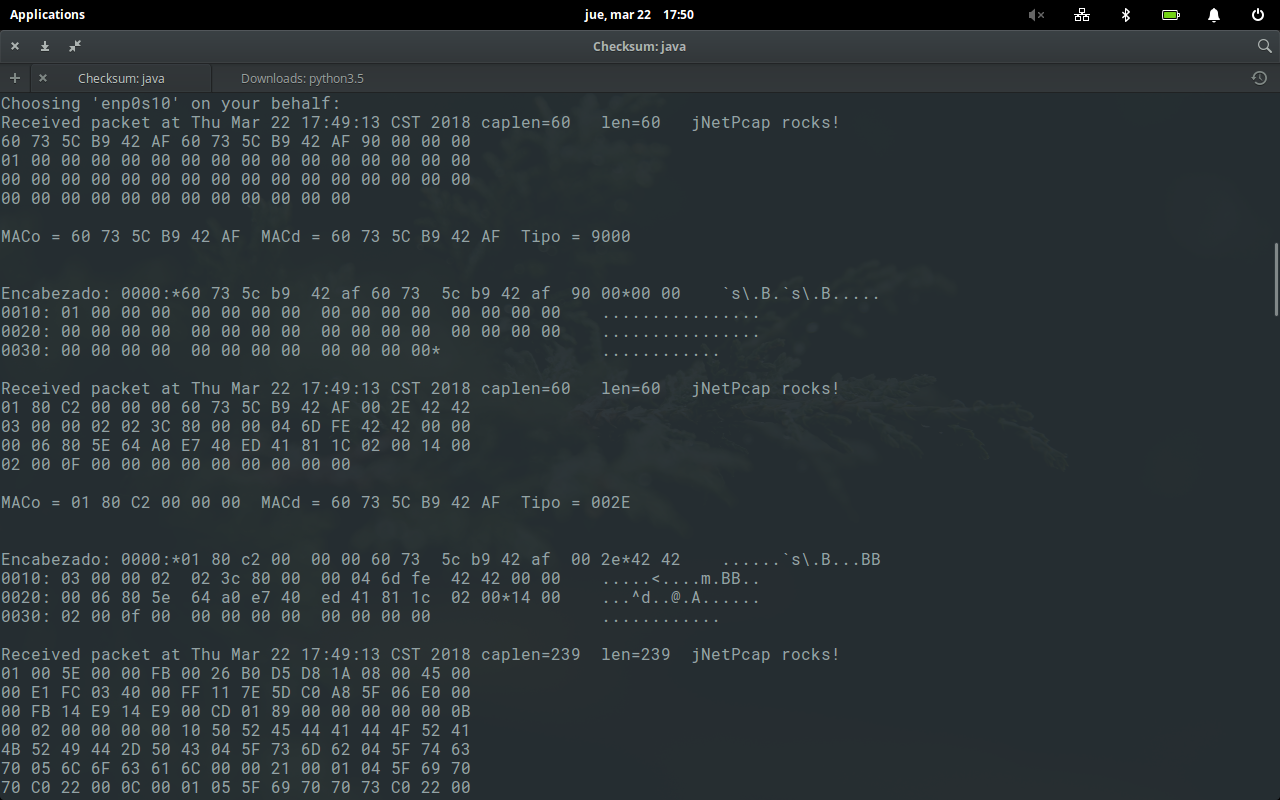
\includegraphics[width=0.85\textwidth]{CheckSum1}

            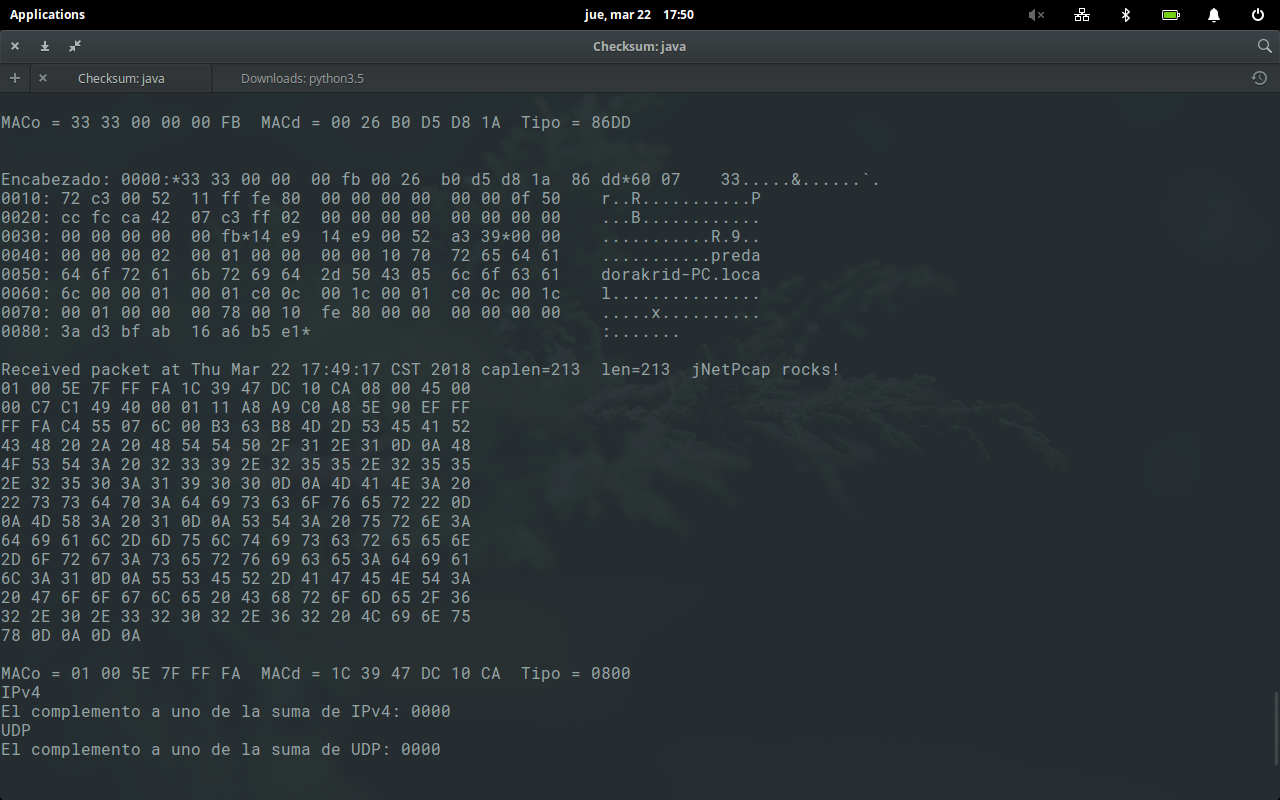
\includegraphics[width=0.85\textwidth]{CheckSum2}
        \end{figure}



    % ===============================================================================
    % ===================          DESARROLLO                  ======================
    % ===============================================================================
    \clearpage
    \section{Código}

        \lstinputlisting[language=Java, linerange={162, 385}, gobble=8]{Code/Checksumv2.java}



    % ===============================================================================
    % ===================          CONCLUSIONES                ======================
    % ===============================================================================
    \clearpage
    \section{Conclusiones}

        \textbf{Arturo Rivas Rojas}: 

            La práctica fue realmente enriquecedora en cuanto a los temas del curso,
            ya que me ayudo a entender mejor sobre la estructura de las tramas Ethernet.

            También por otro lado, me proporciono claridad sobre el principio de encapsulación
            que se debe de cumplir entre cada una de las capas del modelo. 

            Por último, fue interesante el tema de manipulación de la trama como tal para
            aislar el encabezado de los datos, así como para generar el pseudo-header
            necesario para la validación del checksum en TCP y UDP. 

        \textbf{Rosas Hernandez Oscar Andrés}: 

            Es esta práctica implementamos el algoritmo de Checksum aplicado a verificar tramas Ethernet.
            Comprobamos que dichas tramas fueran IPv4 verificando que los bytes 13 y 14 sean iguales a 0x0800,
            para posteriormente decidir si el protocolo de la capa de transporte era TCP o UDP.
            Finalmente, comprobamos el campo checksum de estos protocolos. 

            Al correr el programa, verificamos que varias tramas de TCP llegaban incompletas, por lo
            que el checksum era diferente de cero; mientras que las tramas UDP tendían a llegar sin
            errores la mayoría del tiempo. 

            Lo más importante de esta práctica, es la utilización del algoritmo de checksum para
            identificar los errores en una trama, la cual, asumimos inicialmente, que es una trama Ethernet.

            El checksum se validó con base en el protocolo IPv4 y una vez que se ha dado por buena una trama,
            posteriormente verificamos si el protocolo para el transporte es TCP o UDP, en lo que se utilizó
            el valor calculado del checksum, en el que intervenía un pseudo-header. 

 


\end{document}